%%%%%%%%%%%%%%%%%%%%%%%%%%%%%%%%%%%%%%%%%%%%%%%%%%%%%%%%%%%%%%%%%%%%%%
% LaTeX Example: Project Report
%
% Source: http://www.howtotex.com
%
% Feel free to distribute this example, but please keep the referral
% to howtotex.com
% Date: March 2011 
% 
%%%%%%%%%%%%%%%%%%%%%%%%%%%%%%%%%%%%%%%%%%%%%%%%%%%%%%%%%%%%%%%%%%%%%%
% How to use writeLaTeX: 
%
% You edit the source code here on the left, and the preview on the
% right shows you the result within a few seconds.
%
% Bookmark this page and share the URL with your co-authors. They can
% edit at the same time!
%
% You can upload figures, bibliographies, custom classes and
% styles using the files menu.
%
% If you're new to LaTeX, the wikibook is a great place to start:
% http://en.wikibooks.org/wiki/LaTeX
%
%%%%%%%%%%%%%%%%%%%%%%%%%%%%%%%%%%%%%%%%%%%%%%%%%%%%%%%%%%%%%%%%%%%%%%
% Edit the title below to update the display in My Documents
%\title{Project Report}
%
%%% Preamble
\documentclass[paper=a4, fontsize=11pt, margin=1in]{scrartcl}
\usepackage[T1]{fontenc}
\usepackage{fourier}
\usepackage{longtable}
\usepackage[english]{babel}															% English language/hyphenation
\usepackage[protrusion=true,expansion=true]{microtype}	
\usepackage{amsmath,amsfonts,amsthm} % Math packages
\usepackage[pdftex]{graphicx}	
\usepackage{url}
\usepackage[colorlinks=true]{hyperref}
\usepackage{multicol}
\setlength{\footskip}{120pt}
\usepackage{caption} 
\usepackage{subcaption}

%%% Custom sectioning
\usepackage{sectsty}
\allsectionsfont{\centering \normalfont\scshape}


%%% Custom headers/footers (fancyhdr package)
\usepackage{fancyhdr}
\pagestyle{fancyplain}
\fancyhead{}											% No page header
\fancyfoot[L]{}											% Empty 
\fancyfoot[C]{}											% Empty
\fancyfoot[C]{\thepage}									% Pagenumbering
\renewcommand{\headrulewidth}{0pt}			% Remove header underlines
\renewcommand{\footrulewidth}{0pt}				% Remove footer underlines
\setlength{\headheight}{13.6pt}


%%% Equation and float numbering
\numberwithin{equation}{section}		% Equationnumbering: section.eq#
\numberwithin{figure}{section}			% Figurenumbering: section.fig#
\numberwithin{table}{section}				% Tablenumbering: section.tab#

\setlength{\parindent}{0pt}
%%% Maketitle metadata
\newcommand{\horrule}[1]{\rule{\linewidth}{#1}} 	% Horizontal rule

\title{
		%\vspace{-1in} 	
		\usefont{OT1}{bch}{b}{n}
		\normalfont \normalsize \textsc{University of Maryland Science Academy} \\ [25pt]
		\horrule{0.5pt} \\[0.4cm]
		\huge Using deep learning to predict the temperature of the next 24 hours at the \\
  Ronald Reagan National Airport  \\
		\horrule{2pt} \\[0.5cm]
}
\author{
		\normalfont 								\normalsize
        Sushant Karki\\[-3pt]		\normalsize
        \today
}
\date{}

\setlength{\parindent}{0pt}

%%% Begin document
\begin{document}
\maketitle
\section{\textbf{Abstract}}
Weather forecasts are an integral part of our day-to-day lives. They help us plan ahead and be prepared for the upcoming hours, days and even weeks. We use the weather apps on our phones to check tomorrow's temperature or the chances of rain in order to dress appropriately or to make sure we take our umbrellas with us. These are all weather forecasts that we use regularly without giving a second thought.\\

As it is such an important part of our lives, the accuracy of these forecasts are very important. Not all weather forecasts are made equal as meteorologists use a variety of approaches and a wide range of data to make predictions. \\ 

One emerging approach in the field of weather forecasting is the use of machine learning to make predictions. The abundance of data being collected these days and the increasing advancements in machine learning algorithms make this a task that machine learning is really suited for.\\

This project is an attempt in using machine learning (deep learning in particular) to make hourly weather forecasts for each day at Washington D.C. 

\break

\section{\textbf{Problem Definition and Algorithm}}

\subsection{\textbf{Task Definition: }} 
Using historical hourly weather data of the previous 7 days, predict the temperature for the next 24 hours (12am to next day's 12am).

\subsection{\textbf{Source of Data}}

\textbf{URL:} \href{https://www.wunderground.com/history/daily/us/va/arlington/KDCA/date/2022-12-12}{Wunderground}\\

 Under the hood, Wunderground sends an HTTP request to \textbf{https://api.weather.com} which returns historical hourly data for a particular date and location. \\

 The format of the data is as follows:\\


\begin{longtable}{|p{4.5cm}|p{7cm} |p{3cm}|} % centered columns (4 columns)
\hline\hline %inserts double horizontal lines
\textbf{Field} & \textbf{Description} & \textbf{Example} \\  % inserts table
%heading
\hline
key & Observation weather station ID & KDCA \\
\hline
class & Type of data& observation \\
\hline
expire\_time\_gmt & Expiration time in UNIX seconds & 1669881120 \\
\hline
obs\_id & Observation weather station ID & KDCA \\
\hline
obs\_name & & Washington/Natl \\
\hline
valid\_time\_gmt & Valid time in UNIX seconds. This is the date and time that the observation was made & 1669873920 \\ 
\hline
day\_ind & Time of day of the observation. \newline D = Day \newline N = Night& N \\
\hline
temp & The observed temperature & 42 \\
\hline
wx\_icon & The two-digit number to represent the observed weather conditions. & 33 \\
\hline
icon\_extd & Code representing explicit full set sensible weather & 3300 \\
\hline
wx\_phrase & A text description of the observed weather conditions at the reporting station & \\
\hline
pressure\_tend & The change in the barometric pressure reading over the last hour expressed as an integer. \newline 0 = Steady \newline
1 = Rising or Rapidly Rising \newline
2 = Falling or Rapidly Falling & 0 \\
\hline
pressure\_desc & A phrase describing the change in the barometric pressure reading over the last hour. \newline (Steady, 
Rising, 
Rapidly Rising, 
Falling, Rapidly Falling) & Steady \\ 
\hline
dewPt & The temperature which air must be cooled at constant pressure to reach saturation. The Dew Point is 
also an indirect measure of the humidity of the air. The Dew Point will never exceed the Temperature. 
When the Dew Point and Temperature are equal, clouds or fog will typically form. The closer the values 
of Temperature and Dew Point, the higher the relative humidity. & 60 \\
\hline
heat\_index & An apparent temperature. It represents what the air temperature “feels like” on exposed human skin 
due to the combined effect of warm temperatures and high humidity. 
When the temperature is 70°F or higher, the Feels Like value represents the computed Heat Index. 
For temperatures between 40°F and 70°F, the Feels Like value and Temperature are the same, 
regardless of wind speed and humidity, so use the Temperature value. & 70 \\
\hline
rh & The relative humidity of the air, which is defined as the ratio of the amount of water vapor in the air to 
the amount of vapor required to bring the air to saturation at a constant temperature. Relative humidity 
is always expressed as a percentage. & 91\\
\hline
pressure & Barometric pressure is the pressure exerted by the atmosphere at the earth's surface, due to the weight 
of the air. This value is read directly from an instrument called a mercury barometer and its units are 
expressed in millibars (equivalent to HectoPascals). & 30.06 \\
\hline
vis & The horizontal visibility at the observation point. Visibilities can be reported as fractional values 
particularly when visibility is less than 2 miles. Visibilities greater than 10 statute miles(16.1 kilometers) 
which are considered “unlimited” are reported as “999” in your feed. You can also find visibility values 
that equal zero. This occurrence is not wrong. Dense fogs and heavy snows can produce values near 
zero. Fog, smoke, heavy rain and other weather phenomena can reduce visibility to near zero miles or 
kilometers. & 10 \\
\hline
wc & An apparent temperature. It represents what the air temperature “feels like” on exposed human skin 
due to the combined effect of the cold temperatures and wind speed. 
When the temperature is 61°F or lower the Feels Like value represents the computed Wind Chill so 
display the Wind Chill value. 
For temperatures between 61°F and 75°F, the Feels Like value and Temperature are the same, 
regardless of wind speed and humidity, so display the Temperature value. & -25\\
\hline
wdir & The direction from which the wind blows expressed in degrees. The magnetic direction varies from 1 to 
360 degrees, where 360° indicates the North, 90° the East, 180° the South, 270° the West, and so 
forth.  A ‘null’ value  represents no determinable wind direction. & 45 \\
\hline
wdir\_cardinal & This field contains the cardinal direction from which the wind blows in an abbreviated form. Wind 
directions are always expressed as “from whence the wind blows” meaning that a North wind blows 
from North to South. If you face North in a North wind, the wind is at your face. Face southward and the 
North wind is at your back.
(N , NNE , NE, ENE, E, ESE, SE, 
SSE, S, SSW, SW, WSW, W, 
WNW, NW, NNW, CALM, VAR) & WSW \\
\hline
gust & Wind gust speed. 
This data field contains information about sudden and temporary variations of the average Wind Speed. 
The report always shows the maximum wind gust speed recorded during the observation period. It is a 
required display field if Wind Speed is shown. The speed of the gust can be expressed in miles per 
hour or kilometers per hour.  & 35\\
\hline
wspd & Wind Speed. 
The wind is treated as a vector; hence, winds must have direction and magnitude (speed). The wind 
information reported in the hourly current conditions corresponds to a 10-minute average called the 
sustained wind speed. Sudden or brief variations in the wind speed are known as “wind gusts” and are 
reported in a separate data field. 
Wind directions are always expressed as "from whence the wind blows" meaning that a North wind 
blows from North to South. If you face North in a North wind the wind is at your face. Face southward 
and the North wind is at your back.  & 15 \\
\hline
max\_temp & High temperature in the last 24 hours & 81 \\
\hline
min\_temp & Low temperature in the last 24 hours & 48\\
\hline
precip\_total & Precipitation amount in the last rolling 24 hour period & 0.3 \\
\hline
precip\_hourly & Precipitation for the last hour  & 0.5 \\
\hline
snow\_hourly & Snow increasing rapidly in inches or
centimeters per hour depending on whether
the snowfall is reported by METAR or TECCI
(synthetic observations). METAR snow
accumulation is in inches and TECCI is in
centimeters & 1\\
\hline
uv\_desc & Ultraviolet index description \newline (Extreme, High, Low, Minimal, Moderate, No Report, Not Available)& High \\
\hline
feels\_like & An apparent temperature. It represents what the air temperature “feels like” on exposed human skin 
due to the combined effect of the wind chill or heat index. & 60 \\
\hline
uv\_index & Ultraviolet index \newline (0 to 11 and 999) & 7 \\
\hline
qualifier & Weather description qualifier code & QQ0063 \\
\hline
qualifier\_svrty & Weather description qualifier severity \newline (1 to 6)& 1\\
\hline
blunt\_phrase & Weather description qualifier short phrase & Warmer than yesterday.\\
\hline
terse\_phrase & Weather description qualifier terse phrase & Dangerous wind chills. Limit outdoor exposure. \\
\hline
clds & Cloud cover description code \newline (SKC, CLR, SCT, FEW, BKN, OVC)  & SKC \\
\hline
water\_temp & Water temperature  & 80\\
\hline
primary\_wave\_period & Primary wave period & 13\\
\hline
primary\_wave\_height & Primary wave height & 3.28\\
\hline
primary\_swell\_period & Primary swell period & 13\\
\hline
primary\_swell\_height & Primary swell height & 1.64\\
\hline
primary\_swell\_direction & Primary swell direction & 190\\
\hline
secondary\_swell\_period & Secondary swell period & null\\
\hline
secondary\_swell\_height & Secondary swell height & null\\
\hline
secondary\_swell\_direction & Secondary swell direction & null\\
\hline %inserts single line
\end{longtable}

\subsection{\textbf{Choice of algorithm}}
Since this is a time-series forecasting problem, the Long Short Term Memory (LSTM) neural network was used to build the model. For the look-back period, a period of 7 days(168 hours) were chosen. And since prediction needs to be made for the next 24 hours a multi-step (24 steps) model was trained.\\

A vanilla Recursive Neural Network (RNN) only has a short term memory because it suffers from the vanishing gradients problem. This occurs because during backpropagation in a vanilla RNN, only the recent hidden states are remembered as the gradients for earlier layers get exponentially smaller and don't do much learning at all. An LSTM is much more robust to vanishing gradients and can remember information from earlier inputs much better than a vanilla RNN. \\

My assumption for the prediction problem is that temperature for a particular day not only depends on the day before, but on the weather conditions for a longer timespan (the entire past week). For this reason, LSTM was chosen as it remembers hidden states from the earlier timesteps better.\\

\begin{center}
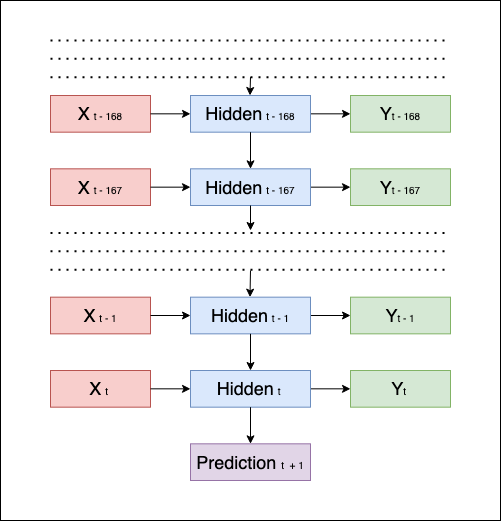
\includegraphics[width=0.8\textwidth,height=0.5\textheight]{lstm.png}
\\
Fig: A simplistic LSTM representation of the modeling task
\end{center}


\section{\textbf{Exploratory Data Analysis}}

22 years worth of historical hourly weather data from 2000-01-01 to 2000-12-06 for the Ronald Reagan National Airport was used for training the model. This amounted to a total of \textbf{247349} rows of weather data records.\\

The first step was to figure out which columns were actually usable in my dataset. For that, I first loaded the data into a pandas DataFrame and checked the NaN counts for each column. I found that almost half of columns were NaN. \\

\begin{center}
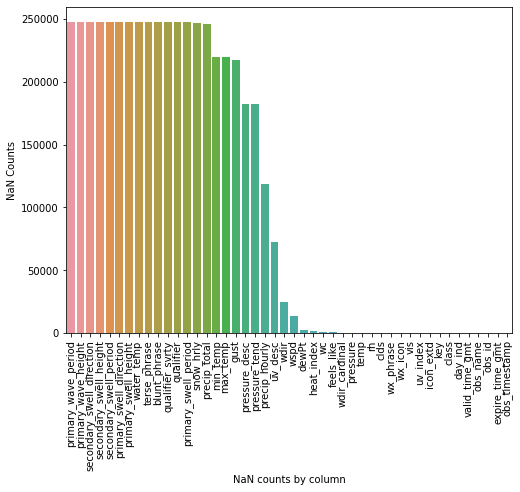
\includegraphics[width=\textwidth]{nan-counts.png}
\end{center}

Using this information, I decided to keep only the following columns (ones that are almost always recorded during observations):\\
\raggedcolumns
\begin{multicols}{4}
\begin{itemize}
\item temp
\item valid\_time\_gmt
\item pressure
\item wspd
\item heat\_index
\item dewPt
\item rh 
\item vis 
\item wc 
\item clds 
\item wdir\_cardinal
\end{itemize}
\end{multicols}

\pagebreak

The next step was to check the columns and see how they were correlated. Just by the column definitions, I knew that heat\_index and wc would be highly correlated to the temperature, but had no idea about how the other columns were related. Using seaborn to plot the correlations, I got the following graph:\\

\begin{center}
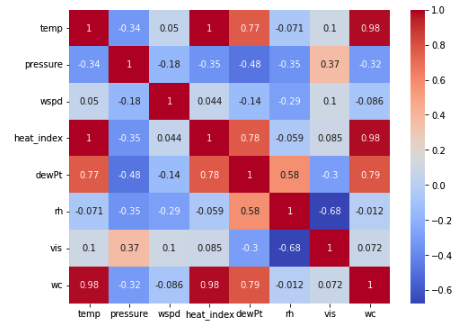
\includegraphics[width=1\textwidth,height=0.5\textheight]{correlations.png}
\\
Fig: Correlation among the columns
\end{center}

Some findings that I took away were that dewPt is highly correlated to the temperature, relative humidity (rh) is highly correlated to the the visibility (vis), and there is also a slight correlation between the pressure and the temperature. 

\section{\textbf{Data Preprocessing}}

Since I want to convert the data into fixed width hourly records, the first step was to convert the UNIX timestamp to a human readable date. This was easily done with the python datetime library.

After converting the unix timestamps into datetime objects, I found that the time the observations are made are not made uniformly. As can be seen from the following screenshot, the observations are not all taken at the same hour.

\begin{center}
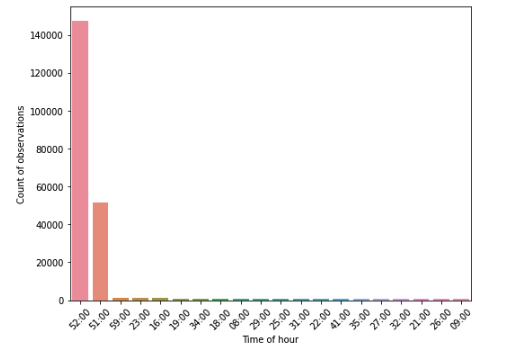
\includegraphics[width=1\textwidth,height=0.5\textheight]{time-of-hour.png}\\
Fig: Graph showing number of observations made at specific minutes of an hour
\end{center}

On further analysis, it became clear that while the observations in first few years of our timespan (2000~2010), the observations were not made at regular intervals, the more recent years had regular intervals. Especially, as evident in the graph above, almost all hourly records had data for the 52\textsuperscript{nd} minute. Thus, I decided to use all the 52\textsuperscript{nd} minute observations as data for our modeling. 

Despite there to be a lot of 52\textsuperscript{nd} minute data in the dataset, I had many missing observations (missing a few hours in some days). Since my LSTM model uses each of the previous 168 hours data as input to make predictions, missing data would cause inaccuracies in my model. To fix this, I used the following interpolations and backfill/forwardfill to fill in the missing rows and created a uniformly spaced timeseries dataframe for training: 

\begin{longtable}{|p{4.5cm}|p{3cm}|p{7cm}|} % centered columns (4 columns)
\hline\hline %inserts double horizontal lines
\textbf{Field} & \textbf{Fill Type} & \textbf{Parameters} \\  % inserts table
%heading
\hline
temp & Interpolation & Polynomial, order=2 \\
\hline
heat\_index & Interpolation & Polynomial, order=2 \\
\hline
pressure & Interpolation & Polynomial, order=2 \\
\hline
wspd & Interpolation & Polynomial, order=2 \\
\hline
dewPt & Interpolation & Polynomial, order=2 \\
\hline
rh & Interpolation & Polynomial, order=2 \\
\hline
wc & Interpolation & Polynomial, order=2 \\
\hline
wdir\_cardinal & Backfill &  \\
\hline
vis & Backfill &  \\
\hline
clds & Interpolation & Linear (Transformed categorical to ordinal and performed interpolation) \\
\hline
\end{longtable}

\begin{center}
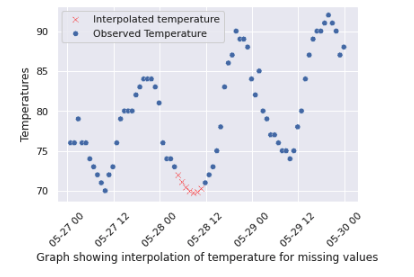
\includegraphics[scale=0.7]{interpolation.png}
\\
Fig: An example of interpolation performed to fill missing 52\textsuperscript{nd} minute temperature values
\end{center}

One big part of predicting weather is to note that weather conditions are cyclical in nature. i.e. weather conditions in January of one year are similar to weather conditions of January of the next year, weather conditions at 1 am today is close distance-wise to weather conditions at 1 am in other days. Directly incorporating the timestamp as a feature would lose this cyclical information. So, I transformed the timestamps (hour of day, day of year) into sin and cosine waves to preserve the cyclical information.

\begin{center}
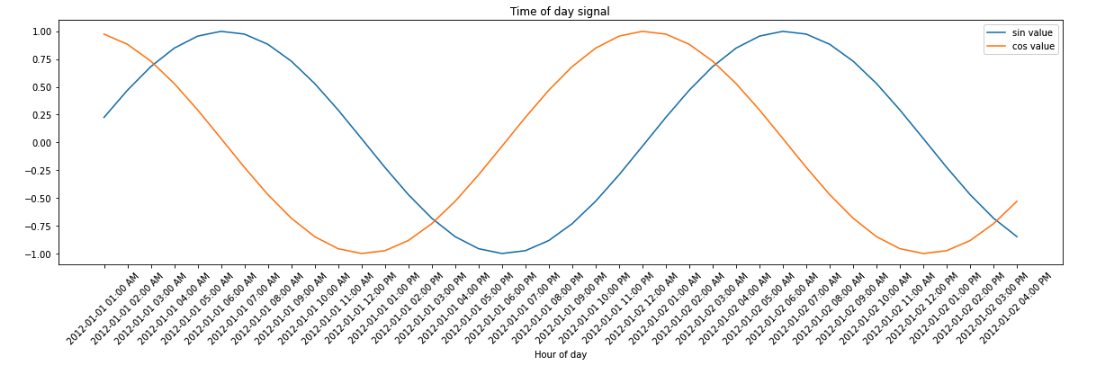
\includegraphics[scale=0.4]{time-of-day.png}
\\
Fig: Hour of day encoded as sine/cosine wave
\end{center}

\begin{center}
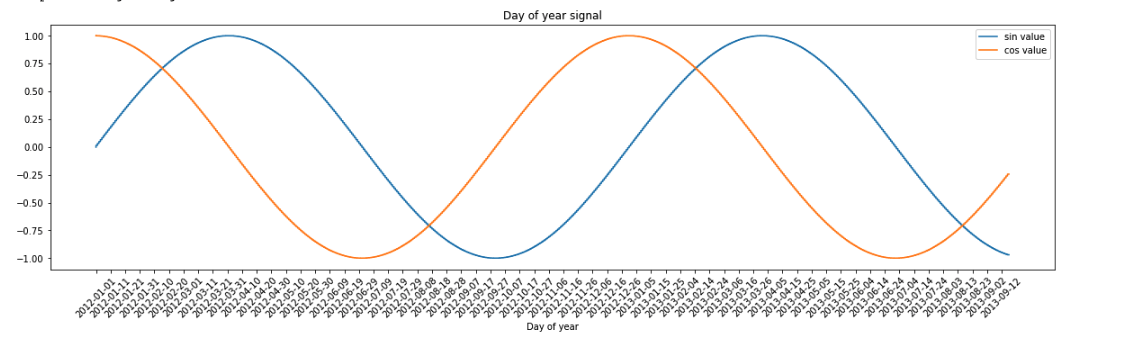
\includegraphics[scale=0.4]{day-of-year.png}
\\
Fig: Day of year encoded as sine/cosine wave
\end{center}

With this, the dataset was ready and I moved on to the training portion of the project.

\pagebreak
\section{\textbf{Training}}

The dataset was split into 70:20:10 train, validation and test sets. 
A StandardScaler was fit into the train dataset and all the train, validation and test sets were standardized with this scaler.

The most crucial step for my model was to generate the sequence of inputs to feed into my LSTM layer. 
Since my approach was to use the last 168 hours of weather data as the lookback for the model, generating the sequence of inputs was a little confusing at first. But thanks to \href{https://www.tensorflow.org/tutorials/structured_data/time_series#data_windowing}{this excellent 
 tensorflow tutorial}, I was able to set it up just right.\\

After generating the sequences, my training data looked like the following:

\begin{center}
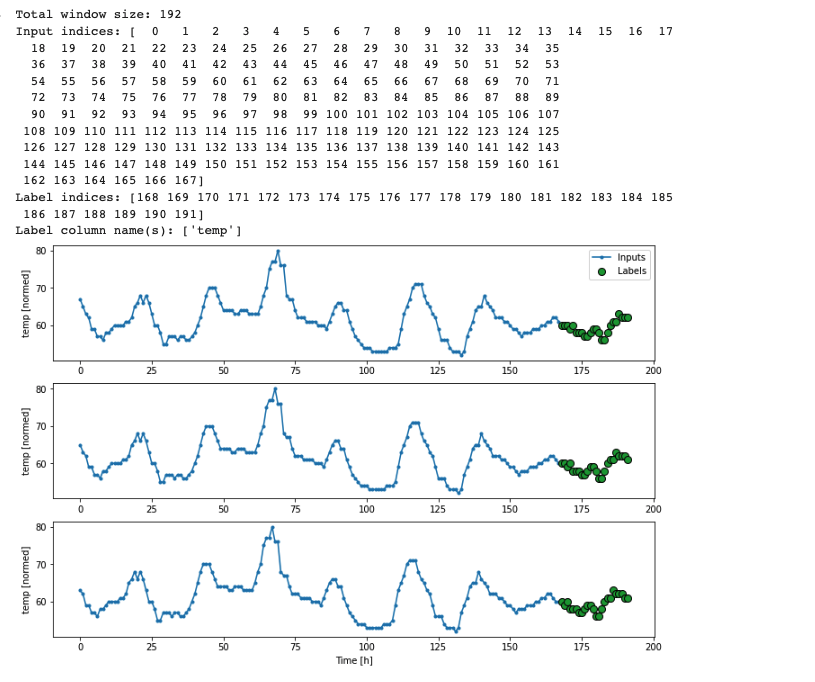
\includegraphics[width=1.2\textwidth]{training-data.png}
\\
Fig: Training Data after sequencing
\end{center}

From the above figure, we can see that for each sample in our training data, the past 168 hours of data have been correctly set up as input features and the next 24 hours have been set aside as labels for training. 

I experimented with stacked LSTM, adding more dense layers, varying LSTM unit counts, and so on. But considering the training time constraints and performance, I found the following model to give the best results for me:

\begin{longtable}{|p{4.5cm}|p{3cm}|p{7cm}|} % centered columns (4 columns)
\hline\hline %inserts double horizontal lines
\textbf{Layer (type)} & \textbf{Output Shape} & \textbf{Param \#} \\  % inserts table
%heading
\hline
\hline
lstm\_2 (LSTM) & (None, 12) & 1248 \\
\hline
dense\_2 (Dense) & (None, 24) & 312 \\
\hline
reshape\_2 (Reshape) & (None, 24, 1) & 0 \\
\hline
\end{longtable}

\begin{longtable}{|p{4.5cm}|}
\hline
\textbf{Total params}: 1,560 \\
\textbf{Trainable params}: 1,560 \\
\textbf{Non-trainable params}: 0\\
\hline
\end{longtable}

\textbf{Framework: } Tensorflow, Keras\\
\textbf{Choice of optimizer:} Adam with learning rate of 1e-3, default decay\\
\textbf{Choice of loss function: } Mean Absolute Error\\
I chose MAE as my loss because it was easier to comprehend and the model converged considerably well for my project. 

\textbf{Max Epochs: } 100 ( I used Early Stopping with a patience of 5 such that if the validation loss didn't go down for 5 straight epochs, the model would stop training further )\\
\\
The model was configured to save every epoch if the validation loss improved from the previous best.

The best model had a validation loss of 3.5005.\\

Although the Mean Absolute Error gave an idea of how accurate my model was, I found it useful to compare it to a baseline model. Thus, for evaluation of my model, I created the following baseline models and trained them on the same dataset:

\begin{center}
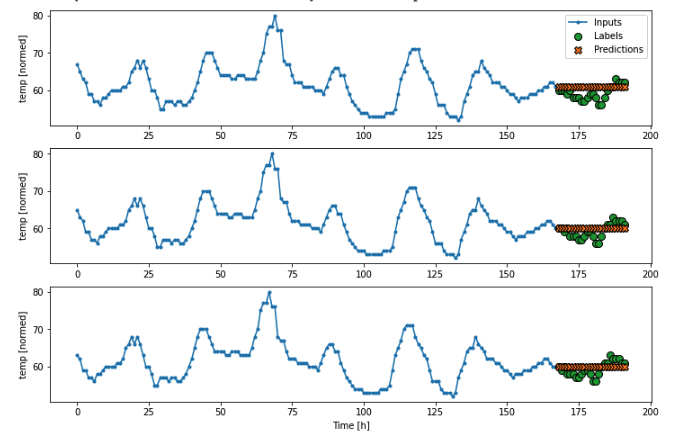
\includegraphics[width=0.93\textwidth]{base-1.png}\\
Fig: Baseline model that predicts a constant temperature no matter what the input.\\
\end{center}

\begin{center}
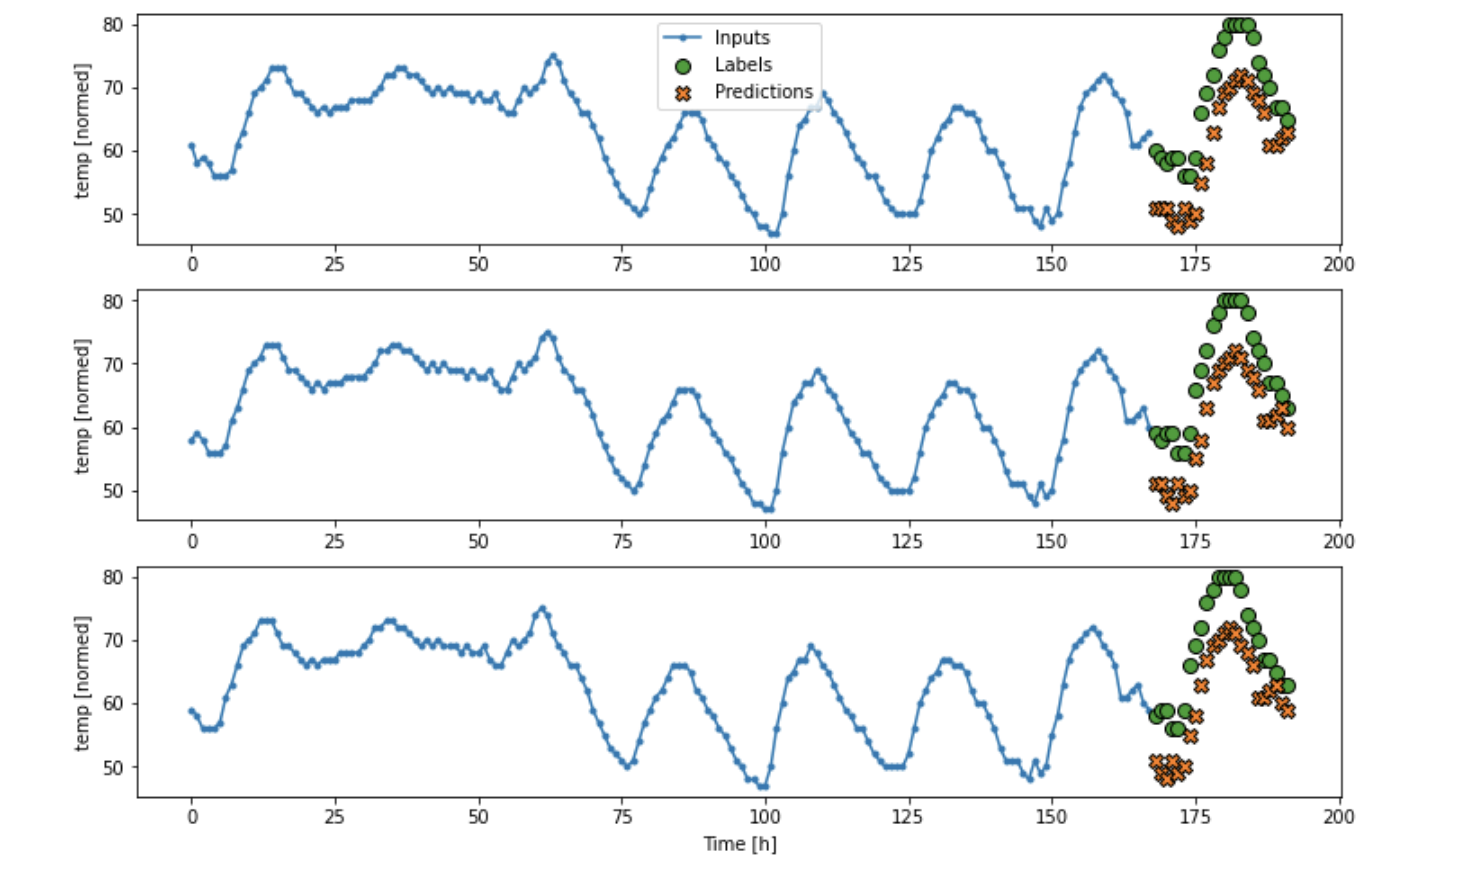
\includegraphics[width=1\textwidth]{base-2.png}\\
Fig: Baseline model that just repeats the previous day's temperatures as predictions 
\end{center}

\pagebreak
Looking at the following graph of the LSTM's performance on test data, it seems that the LSTM model is indeed making more accurate predictions.\\
\begin{center}
    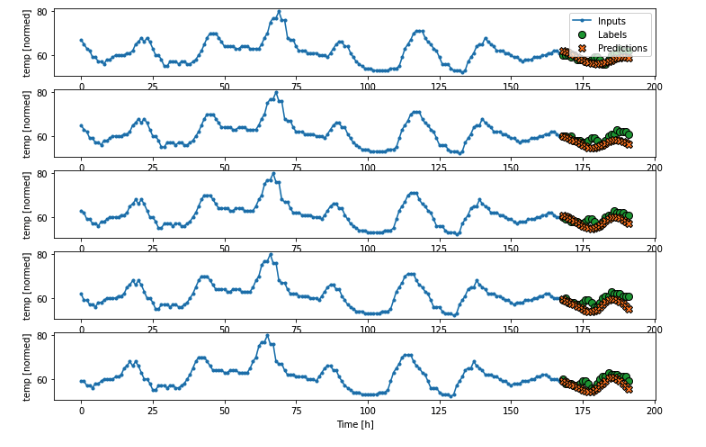
\includegraphics[scale=0.6]{model-eval.png}\\
    Fig: Samples of LSTM model's performance on test dataset\\
\end{center}

Comparing the average Mean Absolute Error for all three models, the following results were seen:\\
\begin{center}
    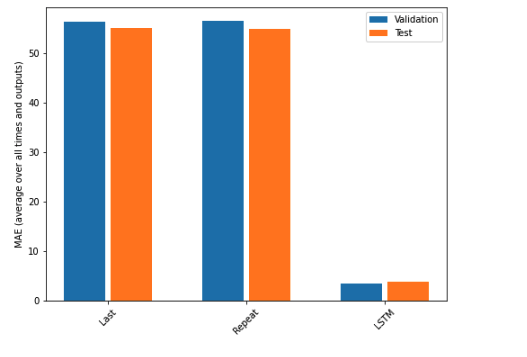
\includegraphics[width=\textwidth,height=0.3\textheight]{comparison.png}\\
    Fig: Comparison of the LSTM model's performance vs the two baseline models
\end{center}

\section{\textbf{Making Predictions / User Interface}}

After building my model, I built a website that uses this model and allows a user to check the model's forecasts for tomorrow's temperature for Washington D.C. The website also shows its past predictions and compares them with the actual temperatures for that day to give a sense of how accurate the model actually is.//

The website is available at \href{http://3.235.0.237/#/dashboard}{\textbf{http\://3.235.0.237/\#/dashboard}}.


\subsection{\textbf{Technology Stack}}


\begin{longtable}{|p{4.5cm}|p{7cm}|} 
\hline
\textbf{Backend} & Flask, Tensorflow \\ 
\hline
\textbf{Frontend} & Angular \\
\hline
\textbf{Infra} & AWS EC2, Docker \\
\hline
\end{longtable}

\subsection{\textbf{Architecture}}
\begin{center}
    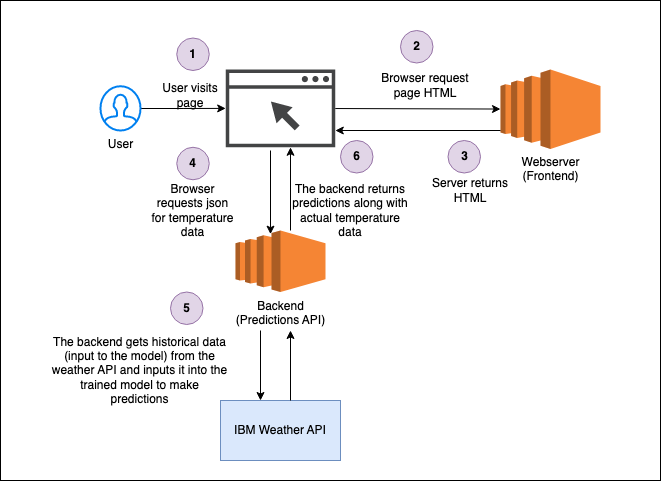
\includegraphics[width=1\textwidth]{weather-requests.drawio.png}\\
    Fig: Request/Response life cycle
\end{center}
\pagebreak

\subsection{\textbf{User Interface}}

The user interface consists of a horizontal scrollable date picker that allows the user to select a date (from the current date to 30 days before the current date) to look at predictions for. The rightmost date is the current date. For the current date, since we don't know the full day actual data yet, the predictions from the model are shown along with the actual temperatures until the time the site is accessed at. The actual temperature for future times will be shown once observation data is available from the weather API.\\

Selecting a date plots the predicted temperature vs the actual temperature for that date in a line graph. The red dotted line indicates the predicted temperature, blue solid one shows the actual temperature for that day. The shaded gray area indicates the absolute error in the prediction. Apart from the graph, the page also contains a tabular view of the same data at the lower half of the page.\\


\begin{center}
    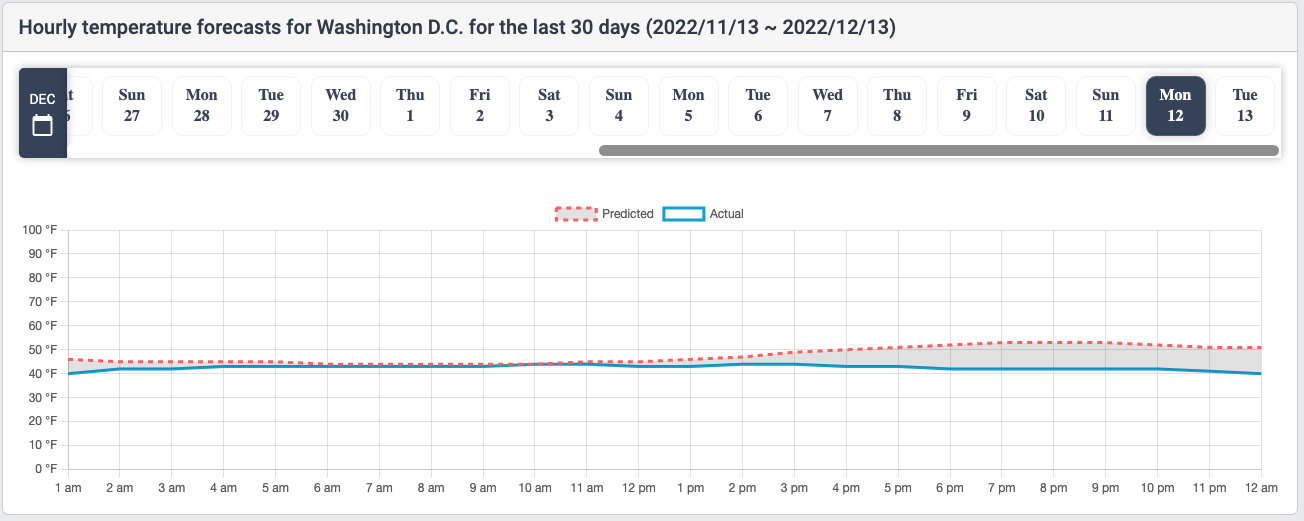
\includegraphics[width=1\textwidth]{graph-view.png}\\
    Fig: Graph View
\end{center}

\begin{center}
    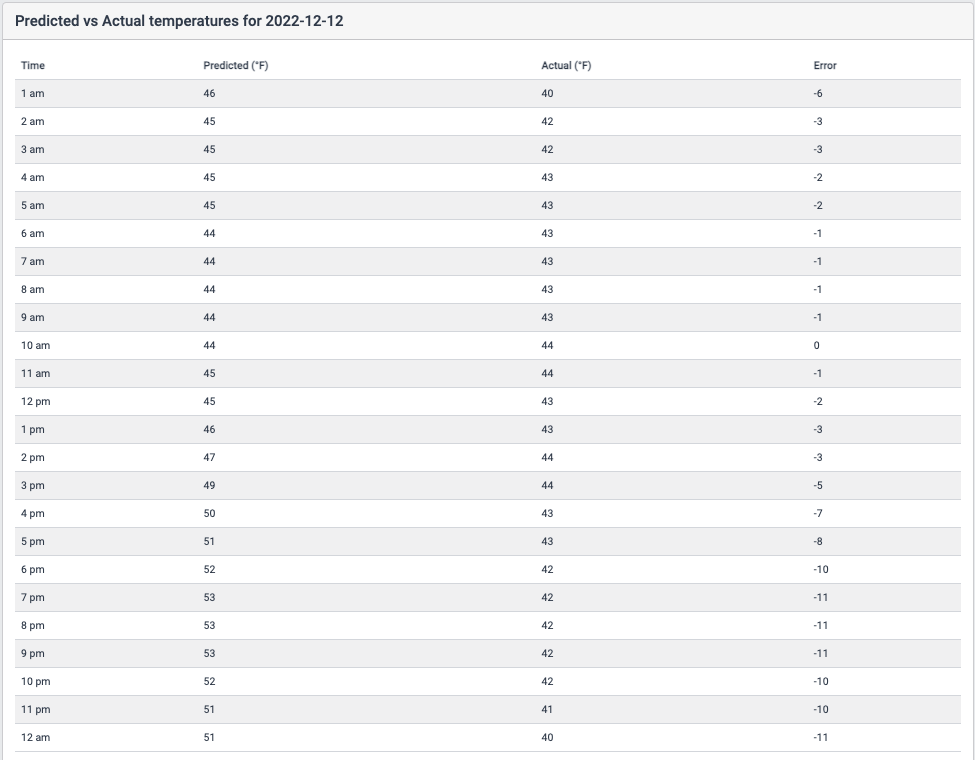
\includegraphics[width=1\textwidth,height=0.3\textheight]{table-view.png}\\
    Fig: Table View
\end{center}

\section{\textbf{Conclusion}}
The final model had a Mean Absolute Error score of about 3.5. i.e. our model's predicted temperatures are about $\pm3.5$ from the actual temperature. Although the accuracy is not as high as I would have liked, looking at the predicted vs the actual temperatures, it seems that the model is capturing the trend (increasing or decreasing) relatively accurately. \\

To improve the model further, I would like to add more important features (perhaps from a completely new dataset) and see how it performs. Although I experimented with the architecture of the neural network, due to time constraints, I wasn't able to experiment as much as I would have liked. So, I definitely want to try different LSTM architectures in the near future and see how they compare to my current model.

\section{\textbf{References}}

\begin{itemize}
    \item Educational Resources 
        \begin{itemize}
            \item \href{https://www.tensorflow.org/tutorials/structured_data/time_series#multi-step_models}{Time series forecasting - Tensorflow}
            \item \href{https://keras.io/examples/timeseries/timeseries_weather_forecasting/}{Timeseries forecasting for weather prediction \- Prabhanshu Attri, Yashika Sharma, Kristi Takach, Falak Shah}
        
            \item \href{https://towardsdatascience.com/single-and-multi-step-temperature-time-series-forecasting-for-vilnius-using-lstm-deep-learning-b9719a0009de}{Single and Multi\-Step Temperature Time Series Forecasting for Vilnius Using LSTM Deep Learning Model, Eligijus Bujokas}
        \end{itemize}
    \item Dataset
        \begin{itemize}
            \item \href{https://www.wunderground.com/}{API: Weather Underground}
            \item \href{https://www.worldcommunitygrid.org/lt/images/climate/The_Weather_Company_APIs.pdf}{Dataset descriptions}
        \end{itemize}
    \item Project Artifacts
        \begin{itemize}
            \item \href{http://3.235.0.237/#/dashboard}{Website URL}
            \item \href{https://colab.research.google.com/drive/1G6E8fT-viMPYw1fnWnBho2ONFfIyAXbK#scrollTo=ykqO9SfV9t7x}{Colab used for training}
            \item \href{https://github.com/00ber/ml-weather-prediction}{Source code}
        \end{itemize}
\end{itemize}

%%% End document
\end{document}
